\section{Zielsetzung}
\label{sec:Zielsetzung}
Im folgenden Versuch sollen mit verschiedenen Scanverfahren ein Acrylblock mit Bohrrungen und ein Brustmodell untersucht werden.
\section{Theorie}
\label{sec:Theorie}
Der für Menschen hörbare Frequenzbereich liegt zwischen 16-20000Hz. Der Bereich unterhalb des hörbaren Bereichs heißt Infraschall. Ultraschall ist der Bereich von 
$\SI{20}{kHz}$ bis $\SI{1}{GHz}$. Oberhalb von $\SI{1}{GHz}$ spricht man von Hyperschall. Ultraschall findet in der Medizin und Werkstoffprüftechnik Anwendung. So kann jener
genutzt werden, um Auskunft über die zu untersuchende Probe zu gewinnen ohne diese zu zerstören.\\
Mathematisch lässt sich Schall als eine longitudinale Welle beschreiben, die sich aufgrund von Druckänderungen durch ein Medium bewegt. Die Beschreibung hat dann die Form
\begin{equation*}
    p(x, t) = p_0 + v_0 Z cos(\omega t - kx).
\end{equation*}
Dabei entspricht $Z = c_M \rho_M$ der akustischen Impedanz. Die Größen $c_M$ und $\rho_M$ sind die Schallgeschwindigkeit und Dichte im Ausbreitungsmedium. Beide sind also
stoffspezifisch.
In Gasen und Flüssigkeiten ist Schall immer eine Longitudinalwelle. Die Schallgeschwindigkeit hängt da von der Dichte $\rho$ und der Kompressibilität $\kappa$ ab. Es gilt:
\begin{equation*}
    c_{Fluessigkeit} = \sqrt{\frac{1}{\kappa \rho}}.
\end{equation*}
In Festkörpern sind aufgrund von Schubspannungen neben Longitudinalwellen auch Transversalwellen möglich. Hier bestimmt das Elastizitätsmodul $E$ die Schallgeschwindigkeit
im Festkörpern, sodass
\begin{equation*}
    c_{Festkoerper} = \sqrt{\frac{E}{\rho}}
\end{equation*}
gilt.
Die Schallgeschwindigkeit der Longitudinalwelle und Transversalwelle kann dabei unterschiedlich groß sein, da Schallgeschwindigkeiten in Festkörpern richtungsabhängig sind.
Durch Absorption nimmt die Intensität der Schallwelle ab. Die Intensität wird dabei mit der Strecke $x$ im Medium skaliert:
\begin{equation*}
    I(x) = I_0 exp(-\alpha x).
\end{equation*}
Dabei ist $I_0$ die anfängliche Intensität und $\alpha$ der Absorptionskoeffizient des Mediums. Bei der Verwendung von Ultraschall nimmt die Amplitude stark durch das 
Durchlaufen von Luft ab. Deshalb wird in der Regel ein Kontaktmittel zwischen Sonde und dem zu untersuchenden Objekt genutzt.\\
\\
Die Ausbreitung von Schall ist ähnlich der einer elektromagnetischen Welle. Bei Grenzflächen zwischen zwei Medien kommt es zur Reflexion und Transmission. Die Welle spaltet 
sich also in einen reflektierten und transmitierten Teil auf. Die Intensität der reflektierten Welle lässt sich mit dem Reflexionskoeffizienten
\begin{equation*}
    R = (\frac{Z_1 - Z_2}{Z_1 + Z_2})^2
\end{equation*}
beschreiben. $Z_1$ und $Z_2$ sind die akustischen Impedanzen des Mediums vor und nach der Grenzfläche. Mit 
\begin{equation*}
    T + R = 1 \Leftrightarrow T = 1 - R
\end{equation*}
lässt sich die transmitierte Intensität berechnen.
\\
\\
Im Experiment wird Ultraschall durch den reziproken piezo-elektrischen Effekt erzeugt. 
Durch ein elektrisches Wechselfeld, das in Richtung einer polaren Achse des Kristalls zeigt, schwingt ein piezoelektrischer Kristall und sendet Ultraschallwellen aus.
Die Schwingungsstärke des Kristalls kann maximiert werden, indem die Anregungsfrequenz der Eigenfrequenz des Kristalls angepasst wird. 
Der Piezokristall kann auch als Schallempfänger dienen, 
indem er durch Schallwellen in Schwingung versetzt wird. Quarze sind die verbreitetsten piezoelektrischen Kristalle, 
weil ihre physikalischen Eigenschaften konstant sind. Der Effekt bei Quarzen fällt jedoch eher schwach aus.\\
\newpage
Um in der Medizin Informationen über den durchstrahlten Körper zu erfahren, werden Laufzeitmessungen von Ultraschall
verwendet. Dazu gibt es zwei geläufige Verfahren:\\
\textbf{1. Durchschallungsverfahren:}\\
Beim Durchschallungsverfahren werden ein Ultraschallsender und -empfänger benötigt. Der Sender senden einen kurzzeitigen
Schallimpuls aus, der durch die Probe propargiert und vom Empfänger aufgefangen wird. An einer Fehlstelle wird eine abgeschwächte Intensität gemessen.
Wie in \autoref{fig:durchschallung} zu sehen, kann keine Aussage über die Tiefe der Fehlstelle getroffen werden,
da der Sender nur sendet und die reflektierten Anteile nicht empfangen kann.\\
\textbf{2. Impuls-Echo-Verfahren:}\\
Anders als beim Durchschallungsverfahren wird beim Impuls-Echo-Verfahren der Sender auch als Empfänger genutzt.
Dadurch kann die Lage der Fehlstelle durch die Laufzeit
\begin{equation*}
    t = \frac{2s}{c} \Leftrightarrow s = \frac{1}{2}ct
\end{equation*}
bestimmt werden. Der ausgesendete Schallimpuls wird an der Grenzfläche der Fehlstelle reflektiert und bei der 
Rückkehr aufgenommen.
\begin{figure}[H]
    \centering
    \begin{subfigure}[b]{0.49\textwidth}
        \centering
        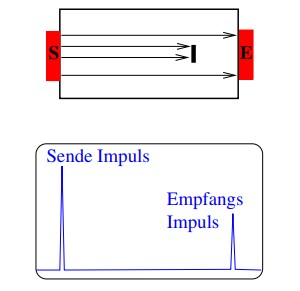
\includegraphics[width=6cm, height=5cm]{img/durchschallung.jpg}
        \caption[]
        {{\small Durchschallungsverfahren}}    
        \label{fig:durchschallung}
    \end{subfigure}
    \hfill
    \begin{subfigure}[b]{0.49\textwidth}  
        \centering 
        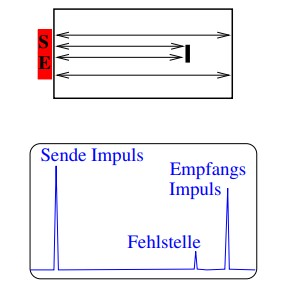
\includegraphics[width=6cm, height=5cm]{img/impulsecho.jpg}
        \caption[]
        {{\small Impuls-Echo-Verfahren.}}    
        \label{fig:impulsecho}
    \end{subfigure}
\end{figure}
Die Laufzeitdiagramme können verschieden dargestellt werden:\\
\textbf{1. A-Scan:}\\
Der Amplitude Scan ist ein eindimensionales Bildgebungsverfahren. Die Intensitätsamplituden werden als Funktion
der Laufzeit aufgetragen. Verwendet wird der A-Scan zur Abtastung von Strukturen.\\
\textbf{2. B-Scan:}\\
Beim Brightness Scan werden die Amplituden in Helligkeitsabstufungen
dargestellt, sodass beim Bewegen der Sonde ein zweidimensionales Schnittbild erzeugt wird.\\
\textbf{3. TM-Scan:}\\
Durch die schnelle Abtastung kann der Time-Motion Scan eine zeitliche Bildabfolge aufnehmen. Damit können dann
z.B. die  Bewegung von Organen aufgenommen werden.\\
